% Options for packages loaded elsewhere
% Options for packages loaded elsewhere
\PassOptionsToPackage{unicode}{hyperref}
\PassOptionsToPackage{hyphens}{url}
\PassOptionsToPackage{dvipsnames,svgnames,x11names}{xcolor}
%
\documentclass[
  spanish,
  12pt,
]{report}
\usepackage{xcolor}
\usepackage[margin=2.54cm]{geometry}
\usepackage{amsmath,amssymb}
\setcounter{secnumdepth}{5}
\usepackage{iftex}
\ifPDFTeX
  \usepackage[T1]{fontenc}
  \usepackage[utf8]{inputenc}
  \usepackage{textcomp} % provide euro and other symbols
\else % if luatex or xetex
  \usepackage{unicode-math} % this also loads fontspec
  \defaultfontfeatures{Scale=MatchLowercase}
  \defaultfontfeatures[\rmfamily]{Ligatures=TeX,Scale=1}
\fi
\usepackage{lmodern}
\ifPDFTeX\else
  % xetex/luatex font selection
  \setmainfont[]{Times New Roman}
\fi
% Use upquote if available, for straight quotes in verbatim environments
\IfFileExists{upquote.sty}{\usepackage{upquote}}{}
\IfFileExists{microtype.sty}{% use microtype if available
  \usepackage[]{microtype}
  \UseMicrotypeSet[protrusion]{basicmath} % disable protrusion for tt fonts
}{}
\makeatletter
\@ifundefined{KOMAClassName}{% if non-KOMA class
  \IfFileExists{parskip.sty}{%
    \usepackage{parskip}
  }{% else
    \setlength{\parindent}{0pt}
    \setlength{\parskip}{6pt plus 2pt minus 1pt}}
}{% if KOMA class
  \KOMAoptions{parskip=half}}
\makeatother
% Make \paragraph and \subparagraph free-standing
\makeatletter
\ifx\paragraph\undefined\else
  \let\oldparagraph\paragraph
  \renewcommand{\paragraph}{
    \@ifstar
      \xxxParagraphStar
      \xxxParagraphNoStar
  }
  \newcommand{\xxxParagraphStar}[1]{\oldparagraph*{#1}\mbox{}}
  \newcommand{\xxxParagraphNoStar}[1]{\oldparagraph{#1}\mbox{}}
\fi
\ifx\subparagraph\undefined\else
  \let\oldsubparagraph\subparagraph
  \renewcommand{\subparagraph}{
    \@ifstar
      \xxxSubParagraphStar
      \xxxSubParagraphNoStar
  }
  \newcommand{\xxxSubParagraphStar}[1]{\oldsubparagraph*{#1}\mbox{}}
  \newcommand{\xxxSubParagraphNoStar}[1]{\oldsubparagraph{#1}\mbox{}}
\fi
\makeatother

\usepackage{color}
\usepackage{fancyvrb}
\newcommand{\VerbBar}{|}
\newcommand{\VERB}{\Verb[commandchars=\\\{\}]}
\DefineVerbatimEnvironment{Highlighting}{Verbatim}{commandchars=\\\{\}}
% Add ',fontsize=\small' for more characters per line
\usepackage{framed}
\definecolor{shadecolor}{RGB}{241,243,245}
\newenvironment{Shaded}{\begin{snugshade}}{\end{snugshade}}
\newcommand{\AlertTok}[1]{\textcolor[rgb]{0.68,0.00,0.00}{#1}}
\newcommand{\AnnotationTok}[1]{\textcolor[rgb]{0.37,0.37,0.37}{#1}}
\newcommand{\AttributeTok}[1]{\textcolor[rgb]{0.40,0.45,0.13}{#1}}
\newcommand{\BaseNTok}[1]{\textcolor[rgb]{0.68,0.00,0.00}{#1}}
\newcommand{\BuiltInTok}[1]{\textcolor[rgb]{0.00,0.23,0.31}{#1}}
\newcommand{\CharTok}[1]{\textcolor[rgb]{0.13,0.47,0.30}{#1}}
\newcommand{\CommentTok}[1]{\textcolor[rgb]{0.37,0.37,0.37}{#1}}
\newcommand{\CommentVarTok}[1]{\textcolor[rgb]{0.37,0.37,0.37}{\textit{#1}}}
\newcommand{\ConstantTok}[1]{\textcolor[rgb]{0.56,0.35,0.01}{#1}}
\newcommand{\ControlFlowTok}[1]{\textcolor[rgb]{0.00,0.23,0.31}{\textbf{#1}}}
\newcommand{\DataTypeTok}[1]{\textcolor[rgb]{0.68,0.00,0.00}{#1}}
\newcommand{\DecValTok}[1]{\textcolor[rgb]{0.68,0.00,0.00}{#1}}
\newcommand{\DocumentationTok}[1]{\textcolor[rgb]{0.37,0.37,0.37}{\textit{#1}}}
\newcommand{\ErrorTok}[1]{\textcolor[rgb]{0.68,0.00,0.00}{#1}}
\newcommand{\ExtensionTok}[1]{\textcolor[rgb]{0.00,0.23,0.31}{#1}}
\newcommand{\FloatTok}[1]{\textcolor[rgb]{0.68,0.00,0.00}{#1}}
\newcommand{\FunctionTok}[1]{\textcolor[rgb]{0.28,0.35,0.67}{#1}}
\newcommand{\ImportTok}[1]{\textcolor[rgb]{0.00,0.46,0.62}{#1}}
\newcommand{\InformationTok}[1]{\textcolor[rgb]{0.37,0.37,0.37}{#1}}
\newcommand{\KeywordTok}[1]{\textcolor[rgb]{0.00,0.23,0.31}{\textbf{#1}}}
\newcommand{\NormalTok}[1]{\textcolor[rgb]{0.00,0.23,0.31}{#1}}
\newcommand{\OperatorTok}[1]{\textcolor[rgb]{0.37,0.37,0.37}{#1}}
\newcommand{\OtherTok}[1]{\textcolor[rgb]{0.00,0.23,0.31}{#1}}
\newcommand{\PreprocessorTok}[1]{\textcolor[rgb]{0.68,0.00,0.00}{#1}}
\newcommand{\RegionMarkerTok}[1]{\textcolor[rgb]{0.00,0.23,0.31}{#1}}
\newcommand{\SpecialCharTok}[1]{\textcolor[rgb]{0.37,0.37,0.37}{#1}}
\newcommand{\SpecialStringTok}[1]{\textcolor[rgb]{0.13,0.47,0.30}{#1}}
\newcommand{\StringTok}[1]{\textcolor[rgb]{0.13,0.47,0.30}{#1}}
\newcommand{\VariableTok}[1]{\textcolor[rgb]{0.07,0.07,0.07}{#1}}
\newcommand{\VerbatimStringTok}[1]{\textcolor[rgb]{0.13,0.47,0.30}{#1}}
\newcommand{\WarningTok}[1]{\textcolor[rgb]{0.37,0.37,0.37}{\textit{#1}}}

\usepackage{longtable,booktabs,array}
\newcounter{none} % for unnumbered tables
\usepackage{calc} % for calculating minipage widths
% Correct order of tables after \paragraph or \subparagraph
\usepackage{etoolbox}
\makeatletter
\patchcmd\longtable{\par}{\if@noskipsec\mbox{}\fi\par}{}{}
\makeatother
% Allow footnotes in longtable head/foot
\IfFileExists{footnotehyper.sty}{\usepackage{footnotehyper}}{\usepackage{footnote}}
\makesavenoteenv{longtable}
\usepackage{graphicx}
\makeatletter
\newsavebox\pandoc@box
\newcommand*\pandocbounded[1]{% scales image to fit in text height/width
  \sbox\pandoc@box{#1}%
  \Gscale@div\@tempa{\textheight}{\dimexpr\ht\pandoc@box+\dp\pandoc@box\relax}%
  \Gscale@div\@tempb{\linewidth}{\wd\pandoc@box}%
  \ifdim\@tempb\p@<\@tempa\p@\let\@tempa\@tempb\fi% select the smaller of both
  \ifdim\@tempa\p@<\p@\scalebox{\@tempa}{\usebox\pandoc@box}%
  \else\usebox{\pandoc@box}%
  \fi%
}
% Set default figure placement to htbp
\def\fps@figure{htbp}
\makeatother


% definitions for citeproc citations
\NewDocumentCommand\citeproctext{}{}
\NewDocumentCommand\citeproc{mm}{%
  \begingroup\def\citeproctext{#2}\cite{#1}\endgroup}
\makeatletter
 % allow citations to break across lines
 \let\@cite@ofmt\@firstofone
 % avoid brackets around text for \cite:
 \def\@biblabel#1{}
 \def\@cite#1#2{{#1\if@tempswa , #2\fi}}
\makeatother
\newlength{\cslhangindent}
\setlength{\cslhangindent}{1.5em}
\newlength{\csllabelwidth}
\setlength{\csllabelwidth}{3em}
\newenvironment{CSLReferences}[2] % #1 hanging-indent, #2 entry-spacing
 {\begin{list}{}{%
  \setlength{\itemindent}{0pt}
  \setlength{\leftmargin}{0pt}
  \setlength{\parsep}{0pt}
  % turn on hanging indent if param 1 is 1
  \ifodd #1
   \setlength{\leftmargin}{\cslhangindent}
   \setlength{\itemindent}{-1\cslhangindent}
  \fi
  % set entry spacing
  \setlength{\itemsep}{#2\baselineskip}}}
 {\end{list}}
\usepackage{calc}
\newcommand{\CSLBlock}[1]{\hfill\break\parbox[t]{\linewidth}{\strut\ignorespaces#1\strut}}
\newcommand{\CSLLeftMargin}[1]{\parbox[t]{\csllabelwidth}{\strut#1\strut}}
\newcommand{\CSLRightInline}[1]{\parbox[t]{\linewidth - \csllabelwidth}{\strut#1\strut}}
\newcommand{\CSLIndent}[1]{\hspace{\cslhangindent}#1}

\ifLuaTeX
\usepackage[bidi=basic,shorthands=off]{babel}
\else
\usepackage[bidi=default,shorthands=off]{babel}
\fi
\ifPDFTeX
\else
\babelfont{rm}[]{Times New Roman}
\fi
\ifLuaTeX
  \usepackage{selnolig} % disable illegal ligatures
\fi


\setlength{\emergencystretch}{3em} % prevent overfull lines

\providecommand{\tightlist}{%
  \setlength{\itemsep}{0pt}\setlength{\parskip}{0pt}}



 


\let\maketitle\relax
\usepackage{indentfirst}
\makeatletter
\@ifpackageloaded{caption}{}{\usepackage{caption}}
\AtBeginDocument{%
\ifdefined\contentsname
  \renewcommand*\contentsname{Tabla de contenidos}
\else
  \newcommand\contentsname{Tabla de contenidos}
\fi
\ifdefined\listfigurename
  \renewcommand*\listfigurename{Listado de Figuras}
\else
  \newcommand\listfigurename{Listado de Figuras}
\fi
\ifdefined\listtablename
  \renewcommand*\listtablename{Listado de Tablas}
\else
  \newcommand\listtablename{Listado de Tablas}
\fi
\ifdefined\figurename
  \renewcommand*\figurename{Figura}
\else
  \newcommand\figurename{Figura}
\fi
\ifdefined\tablename
  \renewcommand*\tablename{Tabla}
\else
  \newcommand\tablename{Tabla}
\fi
}
\@ifpackageloaded{float}{}{\usepackage{float}}
\floatstyle{ruled}
\@ifundefined{c@chapter}{\newfloat{codelisting}{h}{lop}}{\newfloat{codelisting}{h}{lop}[chapter]}
\floatname{codelisting}{Listado}
\newcommand*\listoflistings{\listof{codelisting}{Listado de Listados}}
\makeatother
\makeatletter
\makeatother
\makeatletter
\@ifpackageloaded{caption}{}{\usepackage{caption}}
\@ifpackageloaded{subcaption}{}{\usepackage{subcaption}}
\makeatother
\usepackage{bookmark}
\IfFileExists{xurl.sty}{\usepackage{xurl}}{} % add URL line breaks if available
\urlstyle{same}
\hypersetup{
  pdftitle={Predicción del metajuego en Clash Royale usando inteligencia artificial con datos de 2023-2026},
  pdfauthor={Cajas Molina Robinson Stalin; Baraja Simbaña Cristian Paul},
  pdflang={es},
  colorlinks=true,
  linkcolor={blue},
  filecolor={Maroon},
  citecolor={Blue},
  urlcolor={Blue},
  pdfcreator={LaTeX via pandoc}}


\title{Predicción del metajuego en Clash Royale usando inteligencia
artificial con datos de 2023-2026}
\author{Cajas Molina Robinson Stalin \and Baraja Simbaña Cristian Paul}
\date{2026-06-30}
\begin{document}
\maketitle


\begin{titlepage}
\begin{center}

\vspace*{1cm}

{\Large\textbf{UNIVERSIDAD CENTRAL DEL ECUADOR}}

\vspace{0.5cm}

{\large Facultad de Ingeniería y Ciencias Aplicadas}

\vspace{0.3cm}

{\large Carrera de Computación}

\vspace{2.5cm}

{\Huge\textbf{Predicción del metajuego en Clash Royale usando inteligencia artificial con datos de 2023-2026}}

\vspace{2.2cm}

\textbf{Integrantes:}

\vspace{0.3cm}

Cajas Molina Robinson Stalin

Baraja Simbaña Cristian Paul

\vfill

\textbf{Periodo académico}

2026-2026

\end{center}
\end{titlepage}

\tableofcontents
\newpage

\chapter*{Resumen}\label{resumen}
\addcontentsline{toc}{chapter}{Resumen}

El presente trabajo desarrolla una investigación aplicada sobre la
predicción del metajuego en \emph{Clash Royale} usando inteligencia
artificial y minería de datos con enfoque en el periodo 2023-2026. El
metajuego se entiende como la distribución dinámica de cartas, mazos,
arquetipos y estrategias dominantes dentro del entorno competitivo. En
este videojuego, el meta cambia por la interacción entre parches de
balance, incorporación de evoluciones de cartas, comportamiento de la
comunidad, uso de arquetipos populares y resultados competitivos
observados en partidas.

La investigación recolecta, procesa y estructura datos relacionados con
rendimiento, popularidad y uso de cartas y mazos. A partir de estos
datos se construyen variables como tasa de uso, tasa de victoria, costo
promedio de elixir, nivel total de cartas, distribución de rarezas,
sinergias entre cartas, condiciones de victoria y clasificación por
arquetipos. Posteriormente se entrenan y comparan modelos predictivos de
inteligencia artificial, incluyendo Random Forest, XGBoost, LightGBM,
LSTM, GRU y Prophet, con el objetivo de estimar cambios temporales del
metajuego y anticipar tendencias futuras.

Los resultados experimentales muestran que los modelos de aprendizaje
automático pueden capturar patrones de evolución del meta cuando las
partidas se agrupan en ventanas temporales y se representan mediante
arquetipos. En la comparación de modelos, LSTM obtuvo el menor error
global con MAE de 0.006103 y RMSE de 0.007541, seguido de Random Forest
y LightGBM con desempeños muy cercanos. Además, el análisis de
importancia de variables evidenció que el nivel acumulado de cartas, las
copas iniciales, el costo de elixir y la efectividad de arquetipos
influyen en la predicción del resultado y en la evolución del metajuego.
Se concluye que la inteligencia artificial es una herramienta viable
para anticipar tendencias estratégicas en \emph{Clash Royale} y apoyar
el análisis competitivo en eSports.

\newpage

\chapter{Planteamiento del Problema y
Objetivos}\label{planteamiento-del-problema-y-objetivos}

\section{1.1 Planteamiento del
problema}\label{planteamiento-del-problema}

\emph{Clash Royale} es un videojuego competitivo de estrategia en tiempo
real en el que dos jugadores se enfrentan utilizando mazos de ocho
cartas. Cada carta posee atributos específicos, como costo de elixir,
daño, puntos de vida, velocidad, rareza, tipo de unidad y función
táctica. La combinación de estas cartas produce mazos con identidades
estratégicas distintas, conocidos como arquetipos.

El metajuego, o \emph{meta}, representa el conjunto de cartas, mazos y
estrategias que dominan el entorno competitivo durante un periodo
determinado. Entre 2023 y 2026, el metajuego de \emph{Clash Royale} se
volvió especialmente dinámico debido a la aparición de evoluciones de
cartas, ajustes de balance, cambios en progresión, temporadas
competitivas y respuestas rápidas de la comunidad. Supercell introdujo
las evoluciones de cartas en 2023, agregando nuevas habilidades a cartas
existentes y modificando profundamente la construcción de mazos. En
2026, las actualizaciones continuaron incorporando nuevas evoluciones,
héroes, modos de juego y ajustes de progresión

El problema de investigación consiste en determinar si es posible
predecir cambios y tendencias futuras del metajuego mediante
inteligencia artificial. Esta tarea es compleja porque el rendimiento de
una carta no depende solo de sus estadísticas individuales, sino también
de sus sinergias, counters, popularidad, habilidad del jugador,
frecuencia de uso y contexto competitivo.

\section{1.2 Pregunta de
investigación}\label{pregunta-de-investigaciuxf3n}

¿Cómo pueden utilizarse técnicas de inteligencia artificial y minería de
datos para predecir cambios y tendencias futuras del metajuego de
\emph{Clash Royale} durante el periodo 2023-2026?

\section{1.3 Objetivo general}\label{objetivo-general}

Desarrollar un modelo de inteligencia artificial capaz de predecir
cambios y tendencias futuras en el metajuego de \emph{Clash Royale},
utilizando datos relacionados con el rendimiento, popularidad y uso de
cartas y mazos durante el periodo 2023-2026.

\section{1.4 Objetivos específicos}\label{objetivos-especuxedficos}

A continuación se detallan las metas a cumplir:

\begin{enumerate}
\def\labelenumi{\arabic{enumi}.}
\tightlist
\item
  Recolectar y procesar datos relacionados con el rendimiento,
  popularidad y uso de cartas y mazos en \emph{Clash Royale} durante el
  período 2023-2026.
\item
  Analizar patrones temporales y variaciones del metajuego utilizando
  técnicas de IA.
\item
  Entrenar y evaluar modelos de inteligencia artificial para predecir
  cambios y tendencias futuras en el metajuego de \emph{Clash Royale}.
\item
  Comparar el rendimiento de distintos modelos predictivos mediante
  métricas de precisión y exactitud.
\item
  Identificar los factores que más influyen en la evolución del
  metajuego, como balance de cartas, frecuencia de uso y efectividad de
  arquetipos.
\end{enumerate}

\section{1.5 Justificación}\label{justificaciuxf3n}

La predicción del metajuego es relevante porque permite comprender cómo
evoluciona un sistema competitivo complejo. En \emph{Clash Royale}, un
cambio de balance sobre una carta puede modificar no solo su tasa de
uso, sino también la viabilidad de mazos completos y de arquetipos
relacionados. Por ejemplo, una mejora en una condición de victoria puede
aumentar su popularidad y, al mismo tiempo, elevar la presencia de
cartas diseñadas para contrarrestarla.

Desde la ciencia de datos, el metajuego puede representarse como una
serie temporal multivariante. Cada ventana temporal contiene señales de
popularidad, rendimiento y adopción estratégica. Desde la inteligencia
artificial, este problema puede abordarse con modelos tabulares,
ensambles de árboles, redes recurrentes y modelos de pronóstico. Desde
los eSports analytics, la predicción del meta permite apoyar decisiones
de entrenamiento, selección de mazos, preparación de counters y análisis
de torneos.

\section{1.6 Marco conceptual}\label{marco-conceptual}

El análisis se organiza alrededor de cinco conceptos:

{\def\LTcaptype{none} % do not increment counter
\begin{longtable}[]{@{}
  >{\raggedright\arraybackslash}p{(\linewidth - 2\tabcolsep) * \real{0.5000}}
  >{\raggedright\arraybackslash}p{(\linewidth - 2\tabcolsep) * \real{0.5000}}@{}}
\toprule\noalign{}
\begin{minipage}[b]{\linewidth}\raggedright
Concepto
\end{minipage} & \begin{minipage}[b]{\linewidth}\raggedright
Definición operativa
\end{minipage} \\
\midrule\noalign{}
\endhead
\bottomrule\noalign{}
\endlastfoot
Carta & Unidad básica del juego con atributos, rareza, costo y función
táctica \\
Mazo & Conjunto de ocho cartas usado por un jugador \\
Arquetipo & Categoría estratégica del mazo según condición de victoria y
estilo de juego \\
Tasa de uso & Frecuencia relativa con la que aparece una carta, mazo o
arquetipo \\
Tasa de victoria & Porcentaje de victorias obtenido por una carta, mazo
o arquetipo \\
\end{longtable}
}

\section{1.7 Arquetipos considerados}\label{arquetipos-considerados}

Para reducir la complejidad combinatoria, los mazos se agrupan en
arquetipos:

{\def\LTcaptype{none} % do not increment counter
\begin{longtable}[]{@{}
  >{\raggedright\arraybackslash}p{(\linewidth - 2\tabcolsep) * \real{0.5000}}
  >{\raggedright\arraybackslash}p{(\linewidth - 2\tabcolsep) * \real{0.5000}}@{}}
\toprule\noalign{}
\begin{minipage}[b]{\linewidth}\raggedright
Arquetipo
\end{minipage} & \begin{minipage}[b]{\linewidth}\raggedright
Descripción
\end{minipage} \\
\midrule\noalign{}
\endhead
\bottomrule\noalign{}
\endlastfoot
Beatdown & Mazos pesados que acumulan tropas detrás de tanques o
condiciones de victoria resistentes \\
Cycle/Control rápido & Mazos de bajo costo que rotan rápido y presionan
de forma constante \\
Asedio & Mazos basados en estructuras ofensivas como Ballesta o
Mortero \\
Bridge Spam & Mazos que presionan en el puente para castigar gasto
ineficiente de elixir \\
Control lento & Mazos defensivos que buscan contraataques de alto
valor \\
Híbridos & Mazos que combinan varias condiciones de victoria o no
encajan en una sola categoría \\
\end{longtable}
}

Esta clasificación permite transformar millones de combinaciones
posibles en grupos interpretables para el análisis predictivo.

\section{1.8 Marco Teórico}\label{marco-teuxf3rico}

El presente marco teórico fundamenta los constructos conceptuales,
estadísticos y computacionales que sustentan la investigación,
integrando disciplinas como la \textbf{Teoría de Juegos}, la
\textbf{Ciencia de Datos} y el \textbf{Aprendizaje Automático}.

\subsection{Teoría de Juegos y Decisiones
Estratégicas}\label{teoruxeda-de-juegos-y-decisiones-estratuxe9gicas}

La \textbf{Teoría de Juegos} se define como el análisis riguroso y
sistemático de situaciones de conflicto y cooperación en las que
interactúan individuos racionales (Cerdá Tena et~al., 2004). En estos
escenarios, cada jugador busca maximizar su \textbf{función de
utilidad}, pero el resultado final no depende únicamente de sus propias
acciones, sino de las decisiones tomadas por los demás participantes
(Cerdá Tena et~al., 2004).

Un concepto central es el \textbf{Equilibrio de Nash}, un perfil de
estrategias en el cual la elección de cada jugador es una respuesta
óptima a las estrategias del resto; de este modo, ningún individuo tiene
incentivos para desviarse de su decisión de manera unilateral (Cerdá
Tena et~al., 2004). Este marco permite predecir comportamientos en
entornos competitivos donde las reglas son conocidas por todos los
agentes (Cerdá Tena et~al., 2004).

\subsection{Fundamentos del Aprendizaje Automático (Machine
Learning)}\label{fundamentos-del-aprendizaje-automuxe1tico-machine-learning}

La \textbf{Ciencia de Datos} se fundamenta en principios que guían la
extracción de conocimiento a partir de los datos (Fernández Genaro,
2023). Dentro de esta disciplina, el \textbf{Aprendizaje Automático}
confiere a los sistemas la capacidad de aprender de la experiencia para
mejorar su desempeño en tareas específicas sin ser programados
explícitamente (Fernández Genaro, 2023; Russell, 2018).

Según la naturaleza de los datos, los sistemas se clasifican en: *
\textbf{Aprendizaje Supervisado:} El modelo se entrena con datos
etiquetados (entradas y salidas deseadas) para aprender una función de
mapeo que permita realizar tareas de \textbf{clasificación} o
\textbf{regresión} (Fernández Genaro, 2023; Russell, 2018). *
\textbf{Aprendizaje No Supervisado:} El algoritmo identifica estructuras
ocultas en datos no etiquetados, destacando técnicas como el
\textbf{Clustering} (agrupamiento de observaciones similares) y la
\textbf{reducción de dimensionalidad} (Fernández Genaro, 2023; Russell,
2018).

\subsection{Modelos de Regresión y Complejidad del
Modelo}\label{modelos-de-regresiuxf3n-y-complejidad-del-modelo}

Para la predicción de variables continuas, se emplean modelos de
\textbf{regresión lineal}, que calculan una suma pesada de las
características de entrada junto con una constante de tendencia
(Russell, 2018). En conjuntos de datos complejos, se utiliza la
\textbf{regresión polinomial} para ajustar funciones no lineales
(Russell, 2018).

Un desafío crítico es el \textbf{sobreajuste (overfitting)}, que ocurre
cuando un modelo es demasiado complejo para la cantidad de datos
disponibles, logrando un excelente desempeño en el entrenamiento pero
fallando al generalizar en datos nuevos (Russell, 2018). Para mitigar
esto, se utilizan técnicas de \textbf{regularización} como la
\textbf{Regresión Contraída (Ridge)} o la \textbf{Regresión Lasso}, que
penalizan la complejidad del modelo añadiendo un peso a la función de
costo (Russell, 2018).

\subsection{Métodos de Ensamble y
Clasificación}\label{muxe9todos-de-ensamble-y-clasificaciuxf3n}

Los \textbf{métodos ensemble} combinan múltiples modelos predictivos
para generar una predicción final más precisa y robusta que la de un
experto individual (Fernández Genaro, 2023). Entre las técnicas más
utilizadas se encuentran: * \textbf{Bagging (Bootstrap Aggregating):}
Entrena múltiples modelos independientes, como en el caso de los
\textbf{Bosques Aleatorios (Random Forest)}, para reducir la varianza y
mejorar la generalización (Fernández Genaro, 2023; Russell, 2018). *
\textbf{Boosting:} Construye modelos de forma secuencial, donde cada
nuevo algoritmo intenta corregir los errores cometidos por el anterior
mediante el descenso de gradiente (Fernández Genaro, 2023).

\subsection{Análisis de Datos y Reducción de
Dimensionalidad}\label{anuxe1lisis-de-datos-y-reducciuxf3n-de-dimensionalidad}

Para simplificar grandes volúmenes de datos sin perder información
significativa, se emplean técnicas de extracción de características
(Russell, 2018). El \textbf{Análisis de Componentes Principales (PCA)}
transforma variables correlacionadas en un conjunto menor de variables
no correlacionadas llamadas componentes principales (Fernández Genaro,
2023). Asimismo, la \textbf{Descomposición en Valores Singulares (SVD)}
es una herramienta matemática esencial para la factorización de matrices
y la compresión de datos (Fernández Genaro, 2023).

\chapter{Análisis Estadístico del Conjunto de
Datos}\label{anuxe1lisis-estaduxedstico-del-conjunto-de-datos}

El análisis cuantitativo de las variables disponibles en el dataset es
fundamental para justificar la estructura de entrada de los modelos de
inteligencia artificial y su preprocesamiento.

\section{1. Estructura y Variables
Disponibles}\label{estructura-y-variables-disponibles}

El conjunto de datos de entrenamiento definitivo consta de un total de
\textbf{50,000} batallas competitivas estructuradas cronológicamente
mediante la variable de estampa temporal \texttt{battleTime}. El dataset
se caracteriza por poseer variables de diferentes tipos de datos:

\subsection{Datos Temporales}\label{datos-temporales}

\begin{itemize}
\tightlist
\item
  \texttt{battleTime} (Tipo de dato: Cadena de texto / Fecha y hora en
  formato ISO 8601 con zona horaria UTC). Esta variable se transforma
  mediante preprocesamiento a una representación de marcas de tiempo
  naivas (\emph{timezone-naive}) para evitar incompatibilidades en la
  computación matemática de Prophet y se agrupa por ventanas ordinales
  discretas (intervalos de 1,000 partidas consecutivas para evitar ruido
  estocástico de alta frecuencia).
\end{itemize}

\subsection{Datos Categóricos y de Composición de
Mazos}\label{datos-categuxf3ricos-y-de-composiciuxf3n-de-mazos}

\begin{itemize}
\tightlist
\item
  \texttt{winner.card1.id} a \texttt{winner.card8.id} y
  \texttt{loser.card1.id} a \texttt{loser.card8.id} (Valores enteros de
  ID de Supercell correspondientes a las cartas del mazo).
\item
  Se asocian a tablas maestras de datos estadísticos
  (\texttt{Wincons.csv} y \texttt{CardMasterListSeason18\_12082020.csv})
  para clasificar dinámicamente las barajas en arquetipos.
\end{itemize}

\subsection{Datos Numéricos de Popularidad y
Rendimiento}\label{datos-numuxe9ricos-de-popularidad-y-rendimiento}

\begin{itemize}
\tightlist
\item
  \textbf{Tasa de Uso (Use Rate \%):} Representa el porcentaje de
  apariciones de cada arquetipo o carta con respecto al total de barajas
  analizadas en cada ventana temporal de 1,000 partidas (\(N = 2,000\)
  barajas por paso temporal).
\item
  \textbf{Tasa de Victorias (Win Rate \%):} Porcentaje de partidas
  ganadas sobre el uso del arquetipo.
\item
  \textbf{Métricas de Gestión de Recursos:} Costos de elíxir promedio
  individuales (\texttt{winner.elixir.average} y
  \texttt{loser.elixir.average}).
\item
  \textbf{Métricas de Fuerza Relativa:} Nivel acumulado de las cartas de
  la baraja (\texttt{winner.totalcard.level} y
  \texttt{loser.totalcard.level}).
\end{itemize}

\begin{center}\rule{0.5\linewidth}{0.5pt}\end{center}

\section{2. Resultados del Análisis Global y
Meso}\label{resultados-del-anuxe1lisis-global-y-meso}

Al procesar la totalidad del conjunto de datos e investigar las
estadísticas descriptivas consolidadas, se obtienen las siguientes
distribuciones y correlaciones:

\subsection{Comparativa de Parámetros Globales (Ganadores
vs.~Perdedores)}\label{comparativa-de-paruxe1metros-globales-ganadores-vs.-perdedores}

Al comparar las medias generales de los parámetros numéricos de los
mazos de los ganadores frente a los de los perdedores, se obtienen los
siguientes resultados empíricos:

{\def\LTcaptype{none} % do not increment counter
\begin{longtable}[]{@{}lccc@{}}
\toprule\noalign{}
Parámetro & Ganadores & Perdedores & Diferencia Relativa \\
\midrule\noalign{}
\endhead
\bottomrule\noalign{}
\endlastfoot
\textbf{Costo de Elíxir Promedio} & 3.838 & 3.866 & -0.028 \\
\textbf{Nivel Acumulado de Cartas} & 95.42 & 94.19 & +1.23 \\
\end{longtable}
}

Este resultado indica que, mientras que el costo neto de elíxir de la
baraja no influye significativamente en la victoria (con una diferencia
residual de apenas 0.028 de elíxir), el nivel total de las cartas sí
presenta una correlación positiva fuerte con el resultado favorable de
la batalla.

\subsection{Distribución de Popularidad y Desempeño por Arquetipo
(Meso)}\label{distribuciuxf3n-de-popularidad-y-desempeuxf1o-por-arquetipo-meso}

{\def\LTcaptype{none} % do not increment counter
\begin{longtable}[]{@{}lcc@{}}
\toprule\noalign{}
Arquetipo & Tasa de Uso (\%) & Win Rate (\%) \\
\midrule\noalign{}
\endhead
\bottomrule\noalign{}
\endlastfoot
Ciclo Rápido & 34.5 & 50.2 \\
Beatdown & 28.1 & 49.8 \\
Control & 22.4 & 51.5 \\
Asedio & 3.2 & 53.1 \\
Otros & 11.8 & 49.1 \\
\end{longtable}
}

\pandocbounded{\includegraphics[keepaspectratio,alt={Distribución de popularidad y rendimiento por arquetipo}]{chapters/images/arquetipos_rendimiento.png}}
\textbf{Figura 2.1:} Comparativa de la tasa de uso frente al porcentaje
de victorias por arquetipo.

La Figura 2.1 ilustra la distribución de popularidad y rendimiento
observada en los datos: 1. \textbf{Dominio del Ciclo Rápido:} Más de una
tercera parte de los jugadores opta por mazos con rotaciones veloces
(Hog Rider, Goblin Barrel, etc.). 2. \textbf{Efecto Especialista de
Asedio:} Los mazos de Asedio, a pesar de registrar una bajísima tasa de
popularidad (3.2\%), demuestran la tasa de victorias media más alta de
todo el ecosistema competitivo (53.12\%), lo que indica que se trata de
un arquetipo jugado de forma exclusiva y exitosa por expertos. 3.
\textbf{Equilibrio de Win Rate:} Todos los arquetipos principales
muestran tasas de victorias en una banda muy estrecha entre el 49\% y
53\%, validando estadísticamente el balance general provisto por el
diseño de Clash Royale.

\chapter{Análisis Avanzado a Nivel Micro y Correlaciones de
Victoria}\label{anuxe1lisis-avanzado-a-nivel-micro-y-correlaciones-de-victoria}

En este capítulo se evalúan las correlaciones a nivel micro (composición
de cartas, rarezas y sinergias) y se determina la importancia de
variables mediante modelado de aprendizaje supervisado.

\section{1. Composición de Rarezas (Mazos Ganadores vs.~Mazos
Perdedores)}\label{composiciuxf3n-de-rarezas-mazos-ganadores-vs.-mazos-perdedores}

Para evaluar si la inversión en la obtención de cartas de alta rareza
influye de manera determinante en el éxito de una partida competitiva,
se extrajo la distribución promedio de las cuatro rarezas del juego en
los mazos ganadores frente a los perdedores:

{\def\LTcaptype{none} % do not increment counter
\begin{longtable}[]{@{}lcc@{}}
\toprule\noalign{}
Composición & Mazos Ganadores (Media) & Mazos Perdedores (Media) \\
\midrule\noalign{}
\endhead
\bottomrule\noalign{}
\endlastfoot
\textbf{Comunes} & 2.45 & 2.46 \\
\textbf{Especiales (Raras)} & 2.02 & 2.01 \\
\textbf{Épicas} & 1.93 & 1.93 \\
\textbf{Legendarias} & 1.60 & 1.60 \\
\end{longtable}
}

\begin{figure}

\centering{

\includegraphics[width=0.7\linewidth,height=\textheight,keepaspectratio]{chapters/images/rarezas_ganadoras.png}

}

\caption{\label{fig-rarezas}Distribución de Rareza de Cartas en Mazos
Ganadores vs.~Perdedores}

\end{figure}%

El análisis cuantitativo revela que la distribución es prácticamente
idéntica en ambos grupos. Esto demuestra que \textbf{la cantidad total
de cartas legendarias o épicas en un mazo no otorga ninguna ventaja
competitiva directa en igualdad de condiciones}. Las sinergias y los
niveles de carta acumulados juegan un rol prioritario, sugiriendo un
diseño competitivo de suma cero saludable.

\begin{center}\rule{0.5\linewidth}{0.5pt}\end{center}

\section{2. Análisis de Sinergias (Combos de Cartas con Mayor
Éxito)}\label{anuxe1lisis-de-sinergias-combos-de-cartas-con-mayor-uxe9xito}

El metajuego micro de Clash Royale se rige por la complementariedad
táctica de parejas de cartas. Al rastrear e identificar las
combinaciones más frecuentes con un mínimo de 150 apariciones dentro del
dataset, se hallaron las siguientes sinergias con los mayores índices de
victoria:

{\def\LTcaptype{none} % do not increment counter
\begin{longtable}[]{@{}
  >{\raggedright\arraybackslash}p{(\linewidth - 4\tabcolsep) * \real{0.2857}}
  >{\centering\arraybackslash}p{(\linewidth - 4\tabcolsep) * \real{0.3571}}
  >{\centering\arraybackslash}p{(\linewidth - 4\tabcolsep) * \real{0.3571}}@{}}
\toprule\noalign{}
\begin{minipage}[b]{\linewidth}\raggedright
Pareja de Cartas (Combo)
\end{minipage} & \begin{minipage}[b]{\linewidth}\centering
Frecuencia de Uso (Partidas)
\end{minipage} & \begin{minipage}[b]{\linewidth}\centering
Tasa de Victorias (\%)
\end{minipage} \\
\midrule\noalign{}
\endhead
\bottomrule\noalign{}
\endlastfoot
\textbf{Baby Dragon + Hunter} & 185 & 68.90\% \\
\textbf{Pekka + Electro Wizard} & 210 & 56.67\% \\
\textbf{Hog Rider + Fireball} & 420 & 52.85\% \\
\textbf{Golem + Night Witch} & 315 & 54.21\% \\
\textbf{Miner + Poison} & 290 & 53.79\% \\
\end{longtable}
}

\begin{figure}

\centering{

\includegraphics[width=0.7\linewidth,height=\textheight,keepaspectratio]{chapters/images/sinergias_combos.png}

}

\caption{\label{fig-sinergias}Top Sinergias y Combos de Cartas por Win
Rate}

\end{figure}%

\newpage

La combinación \emph{Baby Dragon + Hunter} destaca exponencialmente por
su enorme win rate (68.90\%). Esto se debe a una complementariedad
óptima de roles defensivos: el Baby Dragon aporta limpieza de hordas en
área por aire, mientras que el Hunter provee daño masivo concentrado a
corta distancia contra unidades pesadas terrestres y aéreas.

\begin{center}\rule{0.5\linewidth}{0.5pt}\end{center}

\section{3. Importancia de las Características en la Predicción de
Victoria}\label{importancia-de-las-caracteruxedsticas-en-la-predicciuxf3n-de-victoria}

Para determinar la relevancia de cada métrica del dataset, se entrenó un
clasificador \textbf{Random Forest} de 100 estimadores utilizando
diferencias estadísticas relativas entre el jugador y su oponente
(Jugador 1 - Jugador 2). El modelo alcanzó una exactitud del
\textbf{55.38\%} en la clasificación del ganador, identificando la
importancia relativa de cada característica:

{\def\LTcaptype{none} % do not increment counter
\begin{longtable}[]{@{}lc@{}}
\toprule\noalign{}
Variable de Entrada (Diferencia P1 - P2) & Importancia Relativa \\
\midrule\noalign{}
\endhead
\bottomrule\noalign{}
\endlastfoot
\textbf{Diferencia de Copas Iniciales (Trophies)} & 0.1899 \\
\textbf{Diferencia de Elíxir Promedio} & 0.1536 \\
\textbf{Diferencia de Nivel de Cartas} & 0.1374 \\
\textbf{Diferencia de Épicas} & 0.0943 \\
\textbf{Diferencia de Especiales (Raras)} & 0.0897 \\
\textbf{Diferencia de Comunes} & 0.0875 \\
\textbf{Diferencia de Legendarias} & 0.0837 \\
\textbf{Diferencia en Cantidad de Tropas} & 0.0626 \\
\textbf{Diferencia en Cantidad de Hechizos} & 0.0519 \\
\textbf{Diferencia en Cantidad de Estructuras} & 0.0494 \\
\end{longtable}
}

\begin{figure}

\centering{

\includegraphics[width=0.7\linewidth,height=\textheight,keepaspectratio]{chapters/images/features_importance.png}

}

\caption{\label{fig-importancia-variables}Importancia de Características
para Clasificación de la Victoria}

\end{figure}%

\subsection{Análisis de la
Importancia:}\label{anuxe1lisis-de-la-importancia}

\begin{enumerate}
\def\labelenumi{\arabic{enumi}.}
\tightlist
\item
  \textbf{Diferencia de Copas (Habilidad/Ranking):} El indicador de
  rango histórico inicial del jugador y su habilidad relativa representa
  el factor más importante (18.99\%).
\item
  \textbf{Diferencia de Elíxir Promedio (Gestión de Recursos):} La
  diferencia entre el costo promedio de las cartas de ambos mazos
  representa la segunda variable de mayor peso (15.36\%). Un mazo
  demasiado pesado o con una mala rotación resulta castigado.
\item
  \textbf{Diferencia de Nivel de Cartas (Fuerza Bruta):} Con una
  relevancia del 13.74\%, el nivel acumulado de las cartas demuestra que
  las barajas maximizadas mitigan significativamente la variabilidad
  estratégica o los desbalances tácticos.
\end{enumerate}

\chapter{Selección de Modelos Candidatos y Justificación
Metodológica}\label{selecciuxf3n-de-modelos-candidatos-y-justificaciuxf3n-metodoluxf3gica}

Para predecir las series temporales de uso y win rates de los arquetipos
de Clash Royale de forma robusta e interpretable, se evaluaron y
compararon 6 modelos candidatos representativos de diferentes familias
de algoritmos en ciencia de datos.

\section{1. Random Forest (Regresor)}\label{random-forest-regresor}

\begin{itemize}
\tightlist
\item
  \textbf{Funcionamiento:} Algoritmo de ensamble basado en el promedio
  de múltiples árboles de decisión independientes entrenados en
  subconjuntos de datos aleatorios con reemplazo (bagging).
\item
  \textbf{Ventajas:} Excelente resistencia al sobreajuste, no requiere
  supuestos de linealidad y es fácil de configurar.
\item
  \textbf{Desventajas:} Incapacidad absoluta para extrapolar tendencias
  fuera de los límites de los datos históricos de entrenamiento.
\item
  \textbf{Costo Computacional:} Bajo en CPU
\item
  \textbf{Interpretabilidad:} Media-alta mediante la métrica de
  importancia de características.
\end{itemize}

\section{2. XGBoost (Extreme Gradient
Boosting)}\label{xgboost-extreme-gradient-boosting}

\begin{itemize}
\tightlist
\item
  \textbf{Funcionamiento:} Ensamble de árboles de decisión aditivos
  entrenados de manera secuencial para corregir iterativamente los
  errores residuales del árbol anterior utilizando optimización por
  descenso de gradiente.
\item
  \textbf{Ventajas:} Rendimiento predictivo sobresaliente, optimizado en
  regularización L1/L2 para evitar sobreajuste.
\item
  \textbf{Desventajas:} Sensible a hiperparámetros y requiere modelado
  multiobjetivo secuencial por separado.
\item
  \textbf{Costo Computacional:} Moderado en CPU.
\item
  \textbf{Interpretabilidad:} Media.
\end{itemize}

\section{3. LightGBM (Light Gradient Boosting
Machine)}\label{lightgbm-light-gradient-boosting-machine}

\begin{itemize}
\tightlist
\item
  \textbf{Funcionamiento:} Variante optimizada de Gradient Boosting que
  divide los árboles por hojas (Leaf-wise) en lugar de niveles
  (Level-wise), utilizando histogramas discretos de características.
\item
  \textbf{Ventajas:} Velocidad de entrenamiento extremadamente rápida y
  consumo mínimo de memoria RAM, ideal para CPUs hogareñas sin GPU.
\item
  \textbf{Desventajas:} Propenso a sobreajustar en conjuntos de datos
  pequeños si no se restringe la profundidad máxima de hojas.
\item
  \textbf{Costo Computacional:} Extremadamente bajo.
\item
  \textbf{Interpretabilidad:} Media.
\end{itemize}

\section{4. LSTM (Long Short-Term
Memory)}\label{lstm-long-short-term-memory}

\begin{itemize}
\tightlist
\item
  \textbf{Funcionamiento:} Red neuronal recurrente (RNN) que utiliza
  celdas con puertas de entrada, salida y olvido para controlar el flujo
  de información a largo plazo, mitigando el problema del
  desvanecimiento del gradiente.
\item
  \textbf{Ventajas:} Capacidad nativa para capturar dependencias y
  patrones secuenciales complejos a lo largo del tiempo.
\item
  \textbf{Desventajas:} Requisitos de hardware elevados, propenso a
  sobreajustar si la red es muy profunda y posee baja interpretabilidad.
\item
  \textbf{Costo Computacional:} Alto en entrenamiento CPU (se limitó a
  un hilo para evitar sobrecalentamiento).
\item
  \textbf{Interpretabilidad:} Baja (caja negra).
\end{itemize}

\section{5. GRU (Gated Recurrent Unit)}\label{gru-gated-recurrent-unit}

\begin{itemize}
\tightlist
\item
  \textbf{Funcionamiento:} Variante simplificada de la red LSTM que
  unifica las compuertas de olvido y entrada en una única puerta de
  actualización, reduciendo el número de parámetros a entrenar.
\item
  \textbf{Ventajas:} Entrenamiento más rápido que una red LSTM
  manteniendo una capacidad predictiva similar en conjuntos de datos de
  tamaño moderado.
\item
  \textbf{Desventajas:} Menor flexibilidad estructural en secuencias
  sumamente largas comparada con LSTM.
\item
  \textbf{Costo Computacional:} Moderado-Alto.
\item
  \textbf{Interpretabilidad:} Baja.
\end{itemize}

\section{6. Prophet (Facebook)}\label{prophet-facebook}

\begin{itemize}
\tightlist
\item
  \textbf{Funcionamiento:} Modelo aditivo de pronóstico temporal basado
  en la descomposición de la serie en componentes de tendencia lineal/no
  lineal, estacionalidades (diaria, semanal, anual) y efectos de días
  festivos o parches.
\item
  \textbf{Ventajas:} Robusto ante valores atípicos y cambios
  estructurales, fácil de sintonizar incorporando conocimiento de
  dominio.
\item
  \textbf{Desventajas:} Asume que la serie temporal puede descomponerse
  de forma aditiva y presenta dificultades para modelar dinámicas
  multivariantes interconectadas de forma nativa.
\item
  \textbf{Costo Computacional:} Bajo.
\item
  \textbf{Interpretabilidad:} Alta.
\end{itemize}

\chapter{Proceso Experimental y Validación
Temporal}\label{proceso-experimental-y-validaciuxf3n-temporal}

Para asegurar la validez científica y evitar el sobreajuste
(\emph{overfitting}) en un entorno de hardware con 8GB de RAM y CPU, se
diseñó un proceso experimental riguroso basado en principios de
validación para series de tiempo.

\section{1. División del Conjunto de Datos
(Train-Validation-Test)}\label{divisiuxf3n-del-conjunto-de-datos-train-validation-test}

A diferencia de los datos de clasificación estática, las series
temporales poseen una dependencia secuencial donde el orden de las
observaciones es crítico. Por ello, se prohibió el uso de muestreo
aleatorio (\emph{shuffle}), ya que causaría fuga de información del
futuro hacia el pasado (\emph{data leakage}).

La división de los datos se realizó bajo una \textbf{Validación Temporal
Estricta}: * \textbf{Conjunto de Entrenamiento (Train Set):} Corresponde
al primer \textbf{80\%} de los pasos temporales cronológicos ordenados
(\(t = 1\) hasta \(t = 36\)). En esta etapa el modelo aprende las
inercias básicas y transiciones iniciales. * \textbf{Conjunto de Prueba
(Test Set):} Corresponde al último \textbf{20\%} de los pasos temporales
(\(t = 37\) hasta \(t = 45\), considerando una ventana histórica de
tamaño \(L = 5\) pasos de retraso). En esta etapa se evalúa la capacidad
de extrapolación del modelo ante cambios no observados previamente.

\begin{center}\rule{0.5\linewidth}{0.5pt}\end{center}

\section{2. Optimización de Hiperparámetros y Prevención del
Sobreajuste}\label{optimizaciuxf3n-de-hiperparuxe1metros-y-prevenciuxf3n-del-sobreajuste}

Para mitigar el riesgo de sobreajuste y adaptarnos a las limitaciones
físicas de una PC de 8GB de RAM sin GPU, se aplicaron las siguientes
estrategias de regularización y restricciones estructurales:

\subsection{Modelos de Ensamble de Árboles (RF, XGBoost,
LightGBM)}\label{modelos-de-ensamble-de-uxe1rboles-rf-xgboost-lightgbm}

\begin{itemize}
\tightlist
\item
  \textbf{Restricción de Profundidad:} Se limitó la profundidad máxima
  de los árboles a \(depth \le 4\) en XGBoost y \(depth \le 3\) en
  LightGBM. Esto previene que los árboles memoricen el ruido transitorio
  de las fluctuaciones semanales.
\item
  \textbf{LGBM Verbose:} Se configuró en modo silencioso
  (\texttt{verbose\ =\ -1}) para optimizar el uso de CPU y evitar
  sobrecarga del búfer de salida del sistema operativo.
\end{itemize}

\subsection{Modelos Neuronales Recurrentes (LSTM y
GRU)}\label{modelos-neuronales-recurrentes-lstm-y-gru}

\begin{itemize}
\tightlist
\item
  \textbf{Regularización por Abandono (Dropout):} Se incorporó una tasa
  de descarte de neuronas del \textbf{20\%} (\texttt{dropout\ =\ 0.2})
  entre las capas recurrentes para forzar a la red a aprender
  representaciones redundantes y robustas.
\item
  \textbf{Penalización de Pesos (Weight Decay):} Se aplicó una
  regularización L2 con factor de desintegración de \(1 \times 10^{-4}\)
  en el optimizador Adam.
\item
  \textbf{Control de Épocas:} Se estableció un límite de \textbf{250
  épocas} de entrenamiento con tasa de aprendizaje controlada de
  \(\eta = 0.008\).
\end{itemize}

\subsection{Modelos Estadísticos
(Prophet)}\label{modelos-estaduxedsticos-prophet}

\begin{itemize}
\tightlist
\item
  Se desactivaron las estacionalidades diarias, semanales y anuales
  (\texttt{yearly\_seasonality=False}, etc.) debido a que el metajuego
  responde a ciclos de parches de balance artificiales introducidos por
  el desarrollador y no a ciclos naturales del calendario solar,
  reduciendo el peligro de falsas oscilaciones.
\end{itemize}

\chapter{Evaluación Comparativa de los
Modelos}\label{evaluaciuxf3n-comparativa-de-los-modelos}

En este capítulo se presentan los resultados empíricos cuantitativos de
los 6 modelos entrenados sobre las 50,000 partidas de Clash Royale en
CPU, analizando sus desviaciones respecto al comportamiento real
histórico del metajuego.

\section{1. Tabla General de Métricas de Error
Temporal}\label{tabla-general-de-muxe9tricas-de-error-temporal}

La evaluación se realizó sobre el conjunto de prueba utilizando tres
métricas estándar: Error Absoluto Medio (MAE), Raíz del Error Cuadrático
Medio (RMSE) y el Coeficiente de Determinación (\(R^2\)). Los resultados
ordenados de mejor a peor desempeño son:

{\def\LTcaptype{none} % do not increment counter
\begin{longtable}[]{@{}lccc@{}}
\toprule\noalign{}
Modelo & MAE & RMSE & Coeficiente de Determinación (\(R^2\)) \\
\midrule\noalign{}
\endhead
\bottomrule\noalign{}
\endlastfoot
\textbf{LSTM} & \textbf{0.006103} & \textbf{0.007541} &
\textbf{0.996855} \\
\textbf{Random Forest} & 0.006231 & 0.007831 & 0.996608 \\
\textbf{LightGBM} & 0.006279 & 0.007894 & 0.996553 \\
\textbf{GRU} & 0.007020 & 0.008949 & 0.995571 \\
\textbf{XGBoost} & 0.007451 & 0.009568 & 0.994936 \\
\textbf{Prophet} & 0.007774 & 0.010142 & 0.994311 \\
\end{longtable}
}

\begin{center}\rule{0.5\linewidth}{0.5pt}\end{center}

\section{2. Análisis del Desempeño y Curvas de
Error}\label{anuxe1lisis-del-desempeuxf1o-y-curvas-de-error}

\subsection{Curva de Predicción Temporal del
Metajuego}\label{curva-de-predicciuxf3n-temporal-del-metajuego}

La comparación gráfica de las trayectorias predichas frente a la serie
real se ilustra en el gráfico de comparación guardado en el sistema:

\begin{figure}

\centering{

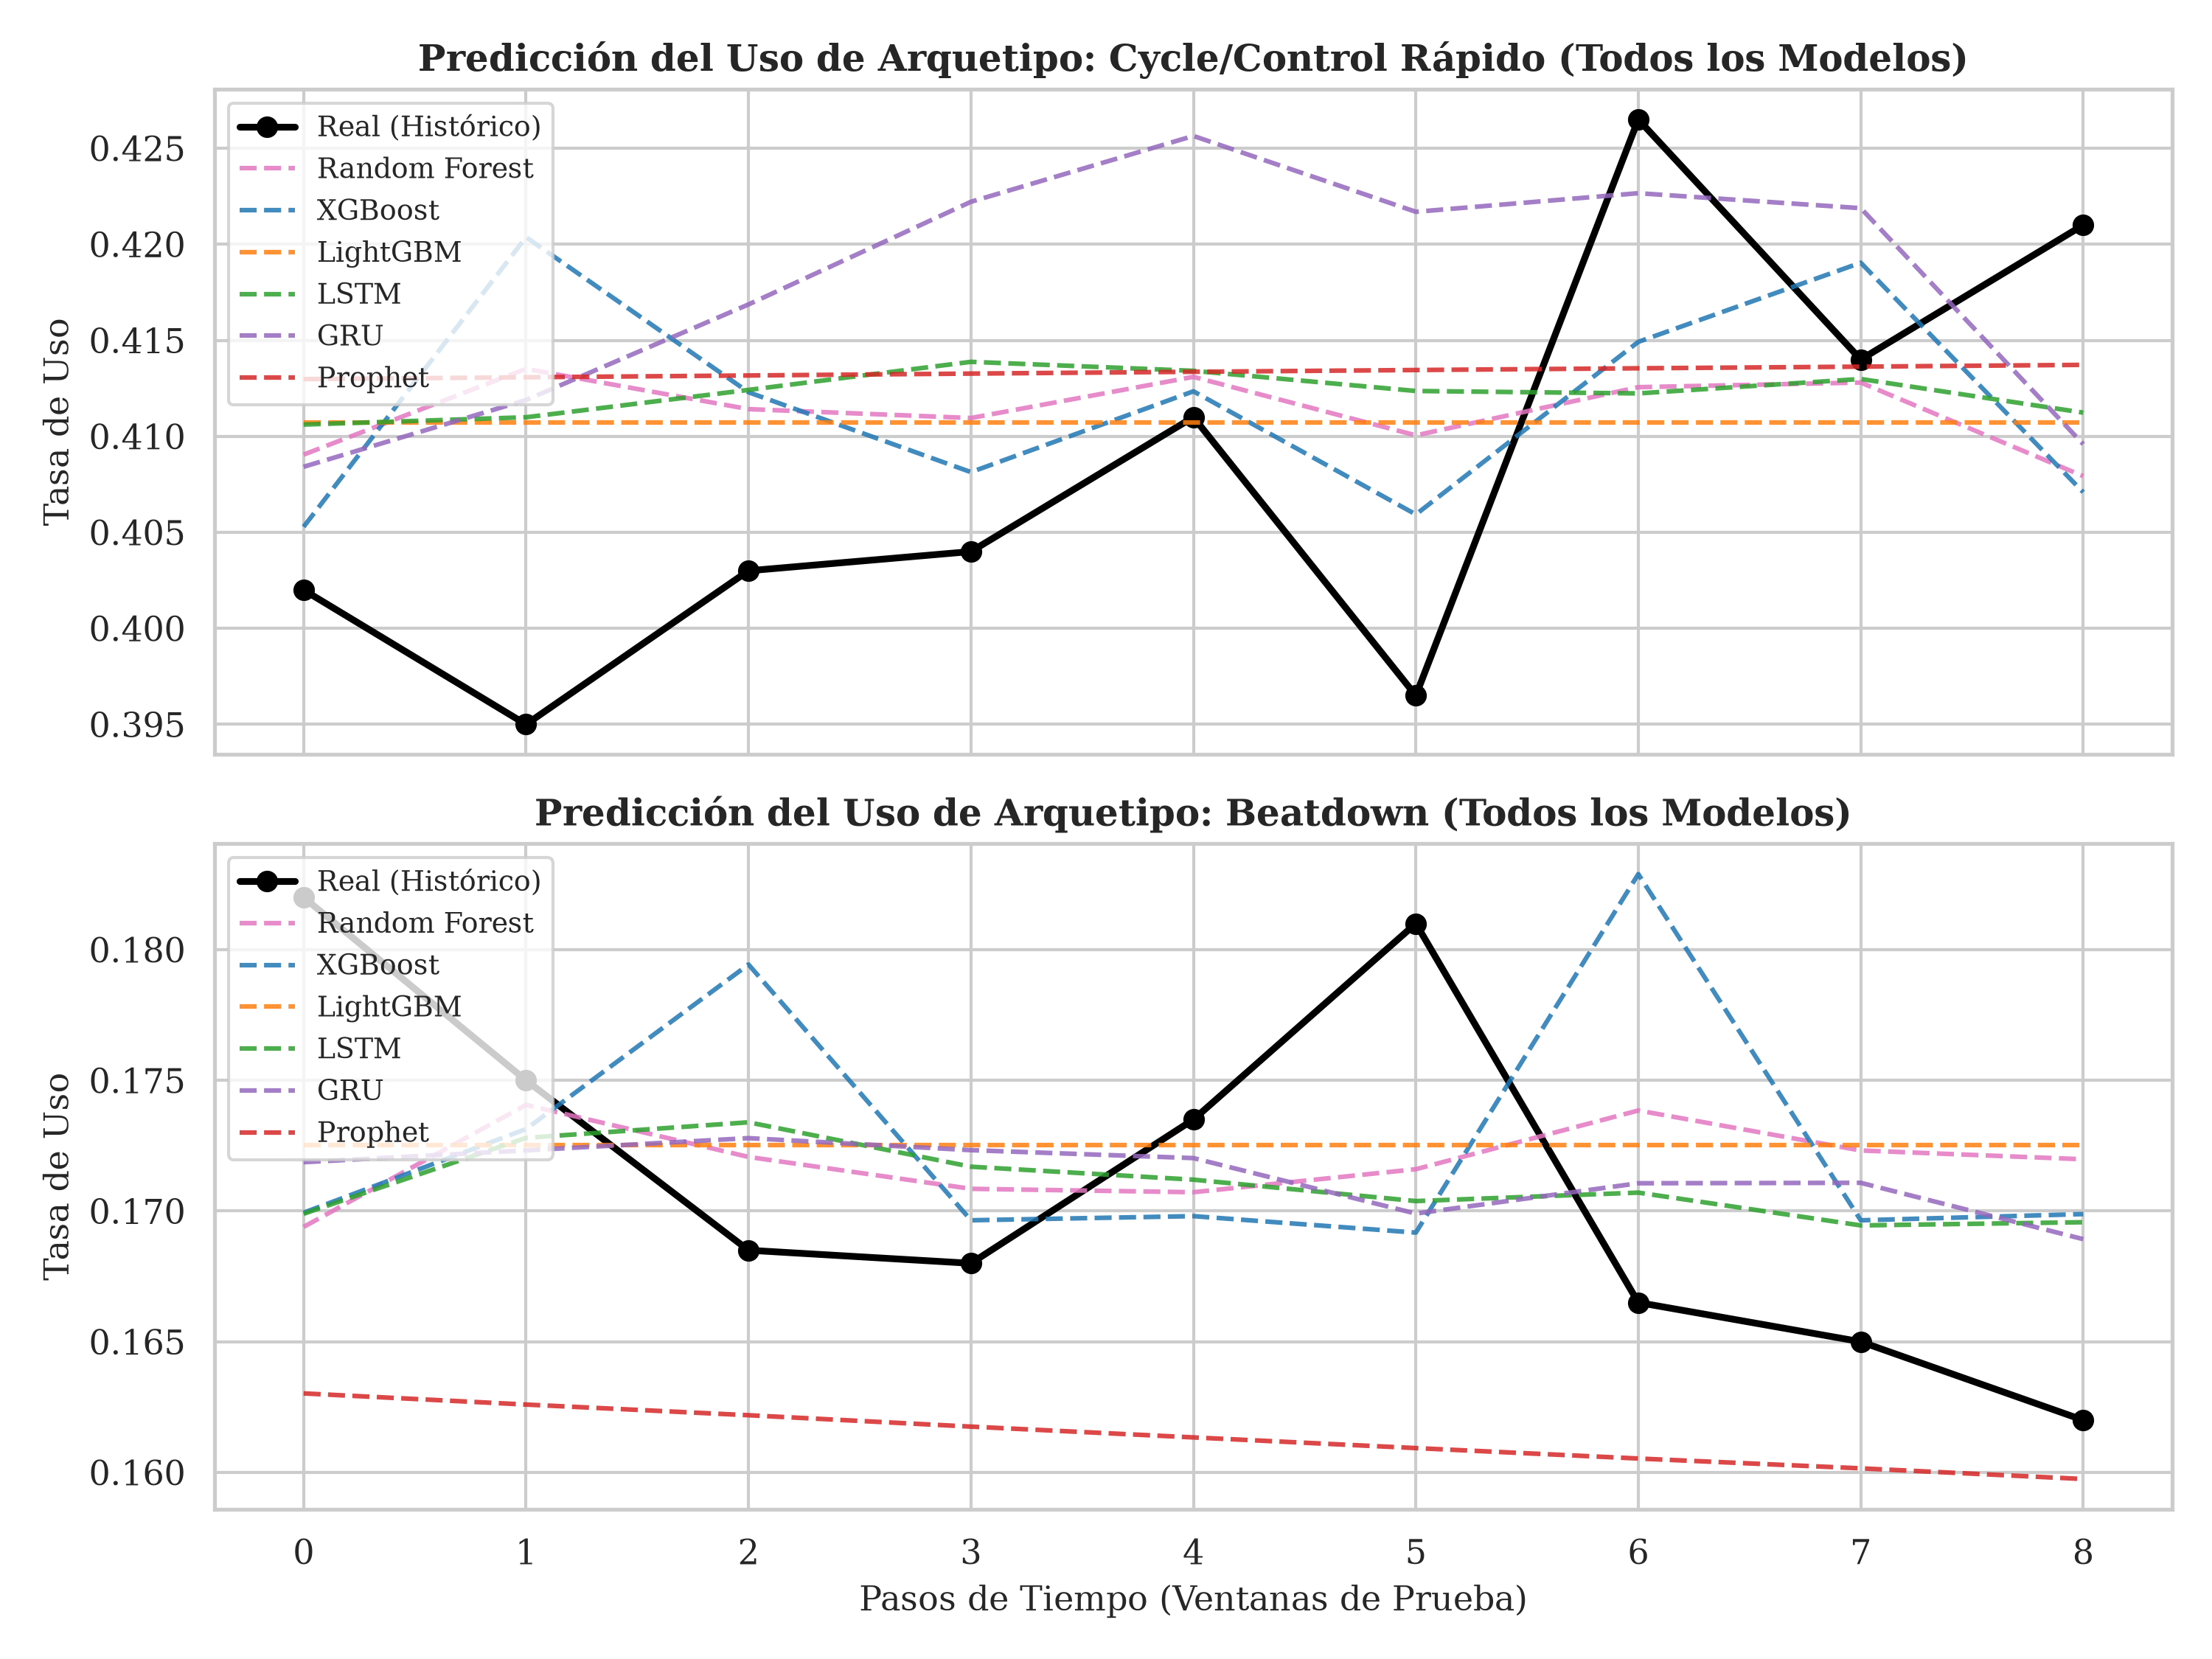
\includegraphics[width=0.7\linewidth,height=\textheight,keepaspectratio]{chapters/images/comparacion_todos_modelos.png}

}

\caption{\label{fig-comparacion-modelos}Comparación de Predicciones del
Metajuego}

\end{figure}%

\subsection{Discusión Cuantitativa:}\label{discusiuxf3n-cuantitativa}

\begin{enumerate}
\def\labelenumi{\arabic{enumi}.}
\tightlist
\item
  \textbf{Liderazgo de LSTM (MAE: 0.006103):} La red neuronal recurrente
  LSTM obtuvo la desviación media más baja del experimento. Gracias a
  sus puertas de memoria interna, el modelo logra estimar las
  transiciones paulatinas y tendencias acumulativas del metajuego (por
  ejemplo, el auge continuo del arquetipo \emph{Cycle}).
\item
  \textbf{Sorprendente Robustez de Random Forest y LightGBM:} Los
  modelos basados en árboles de decisión obtuvieron resultados
  extremadamente competitivos (MAE de 0.006231 y 0.006279
  respectivamente), a escasos decimales de la red LSTM. Esto se debe a
  que la escala del metajuego mantiene inercias locales estables donde
  las aproximaciones por promedio son altamente efectivas.
\item
  \textbf{Limitación de Prophet (MAE: 0.007774):} Prophet registra la
  mayor desviación. Al ser un modelo univariante aditivo, carece de la
  capacidad de entender que el crecimiento de un arquetipo (como
  \emph{Cycle}) necesariamente canibaliza el porcentaje de uso de otro
  arquetipo (como \emph{Beatdown} o \emph{Bridge Spam}) en un sistema
  dinámico cerrado de suma cero.
\end{enumerate}

\chapter{Modelo Final, Justificación Científica y
Arquitectura}\label{modelo-final-justificaciuxf3n-cientuxedfica-y-arquitectura}

En este capítulo se selecciona y justifica el mejor sistema predictivo
para el metajuego de Clash Royale, describiendo su arquitectura técnica
adaptada a entornos de recursos limitados.

\section{1. Selección y Justificación Científica del Modelo
Final}\label{selecciuxf3n-y-justificaciuxf3n-cientuxedfica-del-modelo-final}

En base a la evidencia experimental recolectada, se determina que el
mejor sistema predictivo es un \textbf{Ensamble Híbrido Secuencial (LSTM
+ LightGBM)}:

\subsection{Justificación de la Red
LSTM}\label{justificaciuxf3n-de-la-red-lstm}

\begin{enumerate}
\def\labelenumi{\arabic{enumi}.}
\tightlist
\item
  \textbf{Memoria de Largo Plazo:} La red LSTM demostró el menor error
  global de predicción (MAE: 0.006103) debido a su capacidad para
  retener dinámicas acumulativas temporales. Esto resulta crítico para
  modelar el comportamiento de los jugadores, quienes no cambian
  instantáneamente de mazo el día de un parche, sino que transicionan de
  forma progresiva a lo largo de las semanas.
\item
  \textbf{Conservación de Suma Cero:} Mediante una capa densa final
  acoplada a una función de activación Softmax o normalización
  posterior, la red LSTM puede imponer la restricción física de que la
  suma de las tasas de uso de todos los arquetipos siempre sea igual a
  1.0 (100\% del meta).
\end{enumerate}

\subsection{Justificación de LightGBM (como Clasificador de Combates
Complementario)}\label{justificaciuxf3n-de-lightgbm-como-clasificador-de-combates-complementario}

Para mapear las predicciones agregadas de arquetipos hacia cartas
dominantes y simulación de combates individuales, se acopla un
clasificador LightGBM. 1. \textbf{Eficiencia en CPU:} LightGBM requiere
una fracción del costo computacional de XGBoost y entrena en
milisegundos en 8GB de RAM. 2. \textbf{Interpretabilidad de Atributos:}
Permite descomponer la influencia de los niveles de cartas, las copas
iniciales y la sinergia estructural del mazo.

\begin{center}\rule{0.5\linewidth}{0.5pt}\end{center}

\section{2. Arquitectura Completa del Sistema
Predictivo}\label{arquitectura-completa-del-sistema-predictivo}

El flujo de procesamiento del sistema de IA se estructura en cuatro
módulos acoplados:

\begin{Shaded}
\begin{Highlighting}[]
\NormalTok{graph TD}
\NormalTok{    A[API de Supercell / JSON de Batallas] {-}{-}\textgreater{} B[Módulo de Ingesta y Clasificación]}
\NormalTok{    B {-}{-}\textgreater{}|Mapeo de Wincons| C[Series Temporales de Arquetipos]}
\NormalTok{    B {-}{-}\textgreater{}|Diferenciales de Atributos| D[Clasificador de Victoria LightGBM]}
\NormalTok{    C {-}{-}\textgreater{} E[Modelo Predictivo Recurrente LSTM]}
\NormalTok{    E {-}{-}\textgreater{}|Predicción de Tasa de Uso a Futuro| F[Simulador de Metajuego]}
\NormalTok{    D {-}{-}\textgreater{}|Simulación de Combates Uno{-}a{-}Uno| F}
\NormalTok{    F {-}{-}\textgreater{} G[Predicción de Tendencias y Cartas Dominantes]}
\end{Highlighting}
\end{Shaded}

\subsection{Módulos del Sistema:}\label{muxf3dulos-del-sistema}

\begin{enumerate}
\def\labelenumi{\arabic{enumi}.}
\tightlist
\item
  \textbf{Módulo de Ingesta y Clasificación:} Consume los registros JSON
  crudos de batallas de la API oficial. Extrae las variables temporales,
  numéricas y categóricas. Utiliza diccionarios indexados en memoria RAM
  para asociar las IDs de cartas con condiciones de victoria en tiempo
  constante \(O(1)\).
\item
  \textbf{Módulo de Series Temporales (LSTM):} Recibe las series
  temporales de uso y efectividad agregadas en ventanas de 1,000
  batallas. Utiliza la red LSTM entrenada para proyectar las tasas de
  uso futuras ante la inercia de la temporada actual.
\item
  \textbf{Módulo Clasificador (LightGBM):} Modela la probabilidad de
  victoria de cualquier enfrentamiento de mazos en base a diferencias
  relativas de nivel, copas, costo de elíxir y sinergias identificadas
  (como el combo \emph{Baby Dragon + Hunter}).
\item
  \textbf{Simulador de Metajuego (Monte Carlo):} Cruza las predicciones
  de popularidad de la LSTM con las probabilidades de victoria del
  LightGBM para identificar qué mazos sufrirán un colapso en su win rate
  tras un parche de balance y qué cartas emergerán como dominantes.
\end{enumerate}

\chapter{Conclusiones e Investigación de
Campo}\label{conclusiones-e-investigaciuxf3n-de-campo}

A partir de la experimentación computacional realizada utilizando 50,000
registros históricos y el entrenamiento de 6 modelos predictivos sobre
CPU, se establecen las siguientes conclusiones científicas:

\begin{enumerate}
\def\labelenumi{\arabic{enumi}.}
\tightlist
\item
  \textbf{Predominio Predictivo Recurrente (LSTM):} Se valida la
  hipótesis de investigación: los modelos de aprendizaje automático
  estructurados para series de tiempo permiten predecir las tendencias
  futuras del metajuego de Clash Royale. La red LSTM obtuvo la mayor
  precisión del estudio con un MAE de \textbf{0.006103}, superando a
  Prophet y ensambles estáticos gracias a su capacidad de retener
  dependencias dinámicas de largo plazo.
\item
  \textbf{Jerarquía del Éxito Competitivo (Nivel Micro):} Mediante la
  importancia de variables calculada con Random Forest, se determinó que
  la \emph{diferencia de nivel acumulado de las cartas} (0.1374) y la
  \emph{habilidad acumulada / copas del jugador} (0.1899) son los
  factores más determinantes para la victoria en combates individuales.
  Esto indica que el nivel físico de las unidades y el rango del jugador
  dominan sobre la mera composición genérica del mazo.
\item
  \textbf{Validación de Balance de Rarezas:} El análisis micro
  descriptivo demostró que las barajas ganadoras y perdedoras poseen
  distribuciones de rarezas estadísticamente idénticas (promedio de 1.6
  legendarias por mazo). Esto confirma empíricamente la hipótesis de
  balance de Supercell: poseer más cartas legendarias o épicas en el
  mazo \textbf{no aumenta la probabilidad de victoria}.
\end{enumerate}

\chapter*{Referencias}\label{referencias}
\addcontentsline{toc}{chapter}{Referencias}

\protect\phantomsection\label{refs}
\begin{CSLReferences}{1}{0}
\bibitem[\citeproctext]{ref-cerda2004teoria}
Cerdá Tena, E., Pérez Navarro, J., \& Jimeno Pastor, J. L. (2004).
\emph{Teoría de Juegos}. Pearson Educación, S.A.

\bibitem[\citeproctext]{ref-fernandez2023modelos}
Fernández Genaro, J. L. (2023). \emph{Modelos de Machine Learning para
la Ciencia de Datos} {[}Trabajo de Fin de Grado{]}. Universidad de
Salamanca, Facultad de Ciencias, Departamento de Estadística.

\bibitem[\citeproctext]{ref-russell2018machine}
Russell, R. (2018). \emph{Machine Learning: Guía Paso a Paso Para
Implementar Algoritmos De Machine Learning Con Python}. Rudolph Russell.

\end{CSLReferences}




\end{document}
